\documentclass[12pt]{article}
\usepackage{graphicx}
\usepackage{amsfonts}
\usepackage{amsmath}
\usepackage{fullpage}
\usepackage[utf8x]{inputenc}
\makeatletter
\usepackage{cite}
\usepackage{hyperref}
\@namedef{opt@inputenc.sty}{utf8}
\makeatother
\usepackage{url}
\usepackage{CJKutf8}
\usepackage{multirow}
\usepackage{array}
\newenvironment{conditions}
  {\par\vspace{\abovedisplayskip}\noindent\begin{tabular}{>{$}l<{$} @{${}={}$} l}}
  {\end{tabular}\par\vspace{\belowdisplayskip}}
\begin{document}
\title{
\begin{flushright}

\includegraphics[width=2.5cm]{logoUHi.jpg}\\
{\small
Data Analytics\\
Stiftung Universit{\"a}t Hildesheim\\
Marienburger Platz 22\\
31141 Hildesheim\\
Prof. Dr. Dr. Lars Schmidt-Thieme\\
}
\end{flushright}
\bigskip
\begin{center}
Thesis\\
Unsupervised Real-Time Time-Series Anomaly Detection\\
\end{center}
}
\author{Abdul Rehman Liaqat}
\date{271336, Liaqat@uni-hidesheim.de}
\maketitle

\newpage

\begin{abstract}
Anomaly detection is a crucial task for machine learning due to wide-spread usage and type. In particular, it is worth noting that most data arising in industrial setups are of a streaming nature, thus restricting the range of standard anomaly detection tools. This thesis will identify the potential approaches to learn the identification of abnormal behavior from large-scale streaming data. An empirical comparison of state-of-the-art methods will to be extended by a novel technical contribution. In this thesis, the focus is particularly on streaming time-series Anomaly Detection which changes in nature with time and novel contribution will especially try to target this dynamic nature of time-series.
\end{abstract}
\newpage
\tableofcontents
\newpage
\section{Introduction 10 pages}
\begin{enumerate}
	\item Usage of streaming data		
	\item Usage of anomaly detection in general
	\item Software2.0 development and anomaly detection role
	\item Usage of anomaly detection in streaming data
	\item problems in the concept and brief intro to our innovation
\end{enumerate}
\subsection{Usage of streaming data}
With the increase in networking of objects, amount of data being generated is increasing. A big chunk of this data involves streaming data. Streaming data can be defined as data being generated continuously or with a continuous time interval. Statistically, IoT data has grow from 4.4ZB (Zeta Bytes) to 44.4ZB with 50 billions devices. These devices include a small temperature sensor installed in a room to ECG data to satellite communication data. Even videos are kind of streaming data since they include data points (frames) separated by a constant interval. 
\subsection{Usage of anomaly detection in general}
An anomaly is defined as significantly different data point from other data points. The difference is dependent upon the at least two things. One is the data point being an outlier in general among all data points available. Second is that the data point value doens't make sense in the sequence data is being generated hence it is possible for new data point to be extremely different from all previous ones but still make sense to have in the sequence and vice versa. Detecting an anomaly helps in identifying abnormal behavior of a process with potentially useful information. 
\subsection{Software2.0 development and anomaly detection role}
As described in (reference name Software2), going forward software development especially machine learning based software development will be divided into two parts. One part is the preparation of the data and the second part is the design and optimization of algorithms. Both of these steps are used iteratively. Interestingly, as described in the (reference name Software2), more and more time is spent on accumulating, massaging and cleaning datasets. One major part of this process is outlier detection, anomaly detection and novelty detection. By detection of anomalies, it will become sufficiently easy for human expert to find the one data point in a heap of millions data points and then decide whether to remove that data or get more of the same data points.
Need of an anomaly detection algorithm to identify faulty devices or prevent potential system failure before it happens. Thus the anomaly detection algorithm should be generic (unsupervised), be ready to predict on live data and be able to consider the important past data points (temporal and spatial pattern detection).
\subsection{Usage of anomaly detection in streaming data}
\subsection{problems in the concept and brief intro to our innovation}
Now to define the problem officialy, time series can be defined as an ordered sequence of values of a variable at equally spaced time intervals. It can be a variable or group of variables. For example a heat sensor will be producing one time series which is why it is called univariate time series. If we also consider the output of humidity sensor and noise sensor then the group of these univariate time series will be called multi variate time series. Usually techniques applied on univariate time series can also be used on multivariate after some modification. That's why we will be focusing on univariate time series only in this research thesis. \\
\break
A streaming data or streaming time series has some properties specialized to it. A univariate streaming time series will have following properties:
\begin{enumerate}
	\item Every new data point $x_t$ will be following by a new data point $x_{t+1}$
	\item The time difference between $t - (t-1)*$ and $(t+1) - t$ is approximately the same
	\item There is no known ending time of the stream hence making the streaming data a major source of big data. With this requirement it becomes important to identify important part or time range of the series to be used for the processing.  
\end{enumerate}
Moving on there are some unique concepts related to univariate time series which will be helpful in the understanding of the research problem. Starting with stationay and non-stationary time series. A stationary time series is the one whose statistical properties are constant over time. These statistical properties include mean, variance and autocorrelation of the time series. Similarly with the change in one or more of these statistical properties, non-stationary time series comes into being. These non-stationary time series are also named as Concept drift. Concept drift is a terminology related to time series data specifically which is why we will be using the term Concept drift instead of non-stationary time series in future. There is also an intuitive meaning 
\begin{enumerate}
	\item Stationary and non-stationary time series
	\item lack of labelled data
	\item Amount of diversity hence calling for a universal detector
	\item Concept drift
	\item Points of innovation or constraints to consider for innovation
\end{enumerate}
\newpage
\section{Related Work and State of the art 10 pages}
\begin{enumerate}
	\item Time series intro. Prediction and classification.
	\item Unsupervised methods on time series 
	\item Anomaly detection
	\item Time series Anomaly detection
	\item Unsupervised Time series Anomaly detection
	\item General components latest anomaly detection methods and explanation of each
	\item HTM based anomaly detection paper review. Problems or way it does it
	\item paper 2
	\item paper 3
	\item general review, problems, bottlenecks and trend
\end{enumerate}
\newpage
\section{Proposed method 10 pages}
\subsection{General anomaly score based architecture and detailed explanation}
\begin{figure}
\centering
        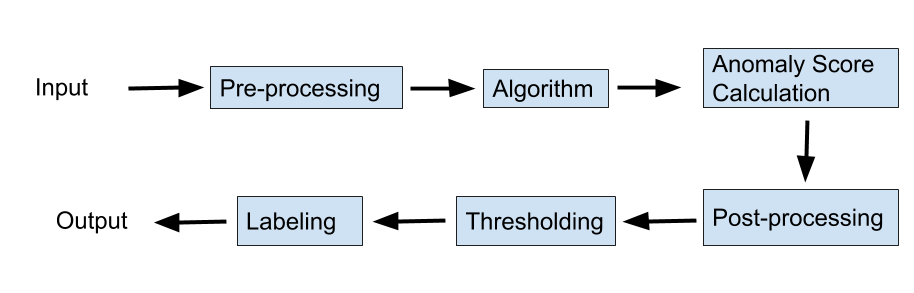
\includegraphics[width=\textwidth]{images/generalAnomalyDetectionFrameWork.png}
    \caption{General Anomaly Detection Framework}
    \label{generalAnomalyDetectionFrameWork}
\end{figure}
Considering figure ~\ref{generalAnomalyDetectionFrameWork}, each algorithm will be using  
all parts with few variations and a cusotmized algorithm part.\\
\break
Pre-processing is playing crucial role in the generalization of the algorithms. There are two different kind of normalization techniques tested. First kind is global normalization
Proposed method can be divided in multiple parts. First part would be the implementation of baselines using latest deep learning architectural components. We use these components to develop two different kind of detectors.\\
\break
One detector is based upon prediction of a next data point. Let $T_{(t-L-1):(t-1)}$ is the small window taken from time series. The starting point is $t-L-1$ where $L$ is the window size and last data point is taken from $t-1$ which is the data point at previous time step. This data window is used to predict the time series value at time $t$. To predict at time $t$ various different kind of functions as baselines using latest architectural components are designed. Generally the output of such a function would be
\begin{equation}
f(T_{(t-L-1):(t-1)}) = \hat{f}(t)
\end{equation} 
Thus the function $f$ in prediction based models map data points as: $f: L \mapsto 1$ where $L$ is the window size and output is the prediction of value at current time. For optimization of function $f$, the difference between time series value at current time step and predicted value at current time is taken. More specifically the objective function will be
\begin{equation}
min |\hat{f}(t) - f(t)|
\end{equation}
That is to minimize the difference between time series value at time $t$ and predicted time series value at time $t$ using time series value from $T_{(t-L-1):(t-1)}$.
\subsection{Describe fully connected prediction architecture}
\subsection{Describe Convolution based prediction architecture}

\subsection{Describe LSTM based prediction architecture}

\subsection{Describe autoencoder based architecture}
\subsection{Describe fully connected based autoencoder based architecture}
\subsection{Describe Convolution based autoencoder based architecture}
\subsection{Describe LSTM based autoencoder based architecture}
\subsection{Recency concept}
\subsection{Post-processing}
\subsection{Thresholding}
\subsection{Parameterinzing the anomaly score}
\newpage 
\section{Empirical Formulation and Experiments 5 pages}
\newpage
\section{Results 10 pages}
\newpage
\section{Conclusion and Discussion 5 pages}
\newpage
\section{Experiment Infrastructure}
\newpage
\subsection{Experiment Management using MLflow}
\newpage
\subsection{Parallel execution using Docker}
\newpage
\section{Best practices}
Following steps were taken to maximize the efficiency and speed of research:
\begin{enumerate}
	\item Use version control to track the code and share between different devices.
	\item Separate code from data. This will keep the code base small and easy to debug.
	\item Separate input data,working data and output data.
	\begin{itemize}
		\item \textbf{Input Data:} Input data-set that never change. For my case it is NAB and other external datasets.
		\item \textbf{Working Data:} nothing for now.
		\item \textbf{Output Data:} Results and threshold profiles in my case. 
	\end{itemize}
	\item Separate options from parameter. This is important:
 	\begin{itemize}
 		\item Options specify how your algorithm should run. For example data path, working directory and result directory path, epochs, learning rate and so on.
 		\item parameters are the result of training data. it includes the score and hyper-parameters. 
 	\end{itemize}
	
\end{enumerate}
\newpage
\subsection{Moving from jupyterlab to pycharm}
While working with jupyterlab notebook following routine was followed:
1- Load data with sample function
2- Write an algorithm
3- Test the results
4- Write general executeable .py file.
5- Get results on server

Since we needed to track change on two different places,
it was becoming harder to track the bugs and improve on efficiency.
That's why pycharm was selected to create executeable files and test
algorithms at the same time.
\section{Reference Usage}
\newpage
\section{References}
\begingroup
\nocite{*}
\renewcommand{\section}[2]{}
\bibliographystyle{IEEEtrans}`
\bibliography{third}
\endgroup
\end{document}
